 
\documentclass{egpubl}
\usepackage{pgv13}

% --- for  Annual CONFERENCE
% \ConferenceSubmission % uncomment for Conference submission
% \ConferencePaper      % uncomment for (final) Conference Paper
% \STAR                 % uncomment for STAR contribution
% \Tutorial             % uncomment for Tutorial contribution
% \ShortPresentation    % uncomment for (final) Short Conference Presentation
%
% --- for  CGF Journal
% \JournalSubmission    % uncomment for submission to Computer Graphics Forum
% \JournalPaper         % uncomment for final version of Journal Paper
%
% --- for  EG Workshop Proceedings
\WsSubmission    % uncomment for submission to EG Workshop
% \WsPaper         % uncomment for final version of EG Workshop contribution
%
 \electronicVersion % can be used both for the printed and electronic version

% for including postscript figures
% mind: package option 'draft' will replace PS figure by a filname within a frame
\ifpdf \usepackage[pdftex]{graphicx} \pdfcompresslevel=9
\else \usepackage[dvips]{graphicx} \fi

\PrintedOrElectronic

\usepackage{t1enc,dfadobe}

\usepackage{egweblnk}
\usepackage{cite}

\title[Visualization of Large Cosmological Data on Hybrid Systems]%
      {Visualization of Large Cosmological Data on Hybrid Systems}

% for anonymous conference submission please enter your SUBMISSION ID
% instead of the author's name (and leave the affiliation blank) !!
\author[M. Rivi \& C. Gheller \& T. Dykes \& I. Cant \& M. Krokos \& K. Dolag]
       {M. Rivi\thanks{Corresponding author}$^{1}$
        and C. Gheller$^{2}$ and T. Dykes$^{3}$ and I. Cant$^3$ and M. Krokos$^{3}$ and K. Dolag$^{4}$
        \\
         $^1$Department of Physics, University of Oxford, United Kingdom\\
         $^2$ETH-CSCS, Lugano, Switzerland\\
         $^3$School of Creative Technologies, University of Portsmouth, United Kingdom\\
         $^4$University Observatory Munich, Germany
       }

% ------------------------------------------------------------------------

% if the Editors-in-Chief have given you the data, you may uncomment
% the following five lines and insert it here
%
% \volume{27}   % the volume in which the issue will be published;
% \issue{1}     % the issue number of the publication
% \pStartPage{1}      % set starting page


%-------------------------------------------------------------------------
\begin{document}

% \teaser{
%  
\includegraphics[width=\linewidth]{eg_new}
%  \centering
%   \caption{New EG Logo}
% \label{fig:teaser}
% }

\maketitle

\begin{abstract}
   The abstract may be up to 3 inches (7.62 cm) long.... 
%   Leave one blank line after the abstract, then add the subject categories according to the ACM Classification Index 

\begin{classification} % according to http://www.acm.org/class/1998/
\CCScat{Programming Techniques}{D.1.3}{Cuncurrent Programming}{Parallel programming}
\CCScat{Computer Graphics}{I.3.7}{Three-Dimensional Graphics and Realism}{Animation}
\CCScat{Simulation and Modeling}{I.6.3}{Applications}
\CCScat{Physical Sciences and Engineering}{J.2}{Astronomy}
\end{classification}

\end{abstract}

 
%-------------------------------------------------------------------------
\section{Introduction}

%-------------------------------------------------------------------------
\section{Visualization of cosmological simulations}

Astrophysicists exploit numerical simulations as an effective instrument to describe, 
investigate and understand the evolution of planets, stars, galaxies and all
the different observed objects and structures 
within the framework of the expanding space-time of the universe. 
There are various numerical methods, grid or particle based, to
perform such simulations. Cluster of galaxies and filamentary structures represent
major topics of investigation. Clusters of galaxies are ideal cosmological probes, being 
the largest collapsed objects in the Universe, hence very sensitive to the structure formation process.
Filaments track the large scale structure of the universe and characterize the 
topology of matter (both dark and baryonic) spatial distribution. Differently from clusters,
filaments are low density objects, hard to detect for the current telescopes. However the interest
around such structures is quicly rising, thanks to the new generations of observational
instruments, like LOFAR or SKA (REF), which can represent suitable tools to trace the filamentary network.

The data produced by numerical simulations require visualisation in order to be fully 
understood, galaxy clusters to be quickly identified and 
their physical properties promptly and effectively displayed and in order 
to figure and conceive the intricated  
connectivity of galaxies, stars and filaments.

In this work, we focus on one of the largest N-body+SPH cosmological simulations
currently available, part of a number of numerical realization known as \textit{Magneticum 
Pathfinder} (REF). Magneticum Pathfinder aims at describing the details of the formation 
of cosmological structures by performing a set of large scale and high resolution simulations, 
taking into account a broad number of physical processes to allow detailed comparison 
to a variety of multi-wavelength observational data. Figure~\ref{fig:pathfinder} summarizes 
the main properties of the different computational boxes simulated in the Pathfinder 
project.

\begin{figure}
\centering
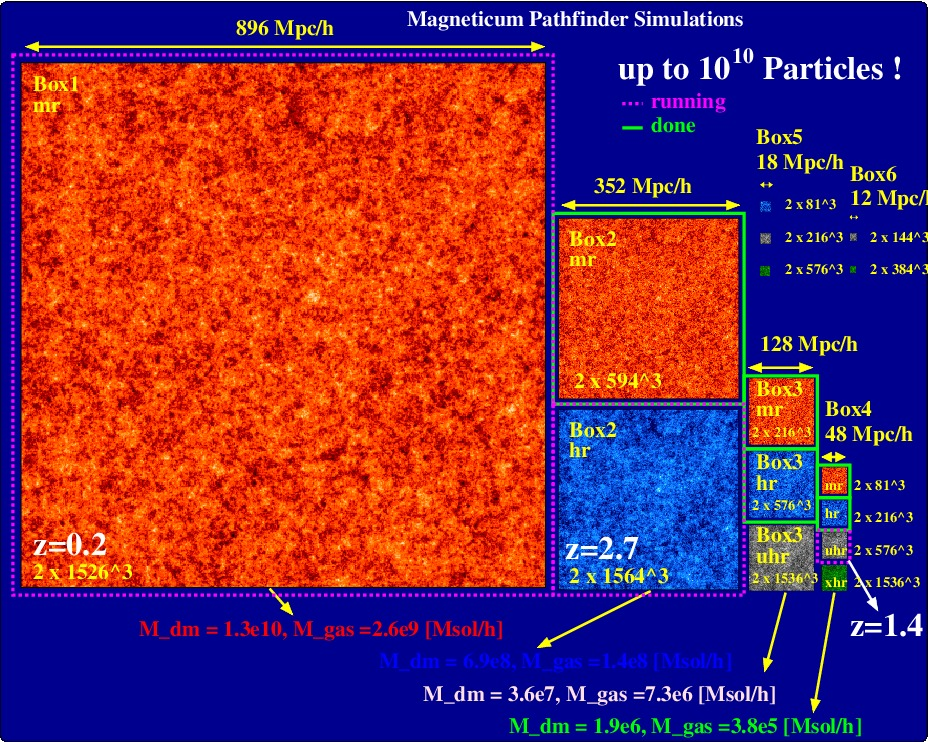
\includegraphics[scale=0.33]{pathfinder.jpg}
\caption{Main details on the different simulations run in the Magneticum 
Pathfinder project.}
\label{fig:pathfinder}
\end{figure}

For all the tests we have used the largest simulation, describing a cubic volume
with side L=1.3 gigaparsec, a representative fraction of the whole universe.
The simulations describes the dark matter component as a set of about four billion particles. The 
same number of fluid elements are used to treat the baryonic component (diffused gas).
More than one billion particles are used to describe the stars. Further five hundred
thousand particles are introduced to describe black holes. Gravity, magneto-hydrodynamics,
cooling and thermal conduction, star formation and chemical enrichment, feedback from
active galaxies are all processes included in the simulation, with corresponding
output variables that can be adopted for visualization (assigning colors or transparencies
to the associated particle species).

The full dataset has been used for all the benchmarks on the HPC system. It has
instead been decimated in order to create a smaller realization to be
used by the previewer for fast exploration and creation of the camera path. The decimation
procedure is simple, since accuracy is not a requirement for the preview stage. It is based on the
extraction of one particle every N. The parameter N is set according to the expected size
of the dataset intended of the previewer. Selected data are saved in a raw binary file.

%-------------------------------------------------------------------------
\section{Splotch: a visualisation tool for astrophysical data}

Splotch (REF WEB) is an open-source, pure C++ code for effectively visualizing large-scale, particle-based datasets. It was designed for visualising N-body and Smoothed Particles Hydrodynamics (SPH) simulations where the data are particles represented by a Gaussian distribution with compact support. However it has also been efficiently used with data defined by regular or adaptive refined meshes by the development of readers able to convert them in the Splotch data type. Several readers are provided supporting a number of popular formats for astrophysics, e.g. HDF5, ...

The rendering algorithm is a derivate of what in general is called volume ray casting and uses an approximation of the radiative transfer equation
which, together with the application of perspective, gives the produced images a very realistic appearance. 

The main strengths of Splotch are high quality of images and the support for large data volumes through an optimised usage of HPC architectures. In fact a parallel version of the code combining the OpenMP and MPI programming paradigms allow to exploit multi-core and multi-node systems~\cite{JKR*10}. Moreover a CUDA version of the code is also available to accelerate the computation on GPUs~\cite{RGD*14}. 

Another important characteristic of this tool is its high level of customisation, through a parameter file, to suit specialised scientific dataset. To help the user in the fine tune of the parameters required by Splotch a Previewer tool is available (see Section~3).

%-------------------------------------------------------------------------
\subsection{Algorithm overview }

The operational scenario~\cite{DRGI08} consists in two main stages after reading particles from single or multiple data files. 
In the first stage, that we call \textit{rasterization}, a preprocessing step can perform ranging, normalization, and apply logarithms to particle attributes if required. Then particle coordinates and their \textit{smoothing length} $\sigma_p$ (i.e. the standard deviation of the gaussian distribution $\rho_p(x)$ describing the particle) are roto-translated, with reference to supplied camera and look-at positions, and projected according to a given field of view. Finally particles falling in the scene are identified and assigned with RGB colour values via a colour look-up table or palette (which can be provided as an external file).

The final stage is \textit{rendering}, where rays originating from each pixel of the image are cast along lines of sight, and contributions of all encountered particles are accumulated. The contribution of particles is determined by solving the radiative transfer equation:
\begin{equation}\label{rad}
 \frac{d I(x)}{dr}=( E_p- A_p I(x))\rho_p(x),
\end{equation}
where $I(x)$ is the colour intensity at position $x$, $E_p$ and $A_p$ describe the strength of radiation emission and absorption of particle $p$ for the three RGB colour component.

%-------------------------------------------------------------------------
\subsection{MPI+CUDA implementation}
The MPI implementation~\cite{JKR*10} simply distributes chunks of particles among different processors, each performing independently a serial computation and producing a partial rendering. The final image is composed by a collective reduction operation and saved only by the root processor.

By enabling the usage of GPUs, each MPI tasks executes the CUDA version of the code described in~\cite{RGD*14} to render its chunk of particles. 
Summarizing, each task transfers its data (or sub chunks of it a time if necessary) to the global GPU memory, then each particle is processed by the Rasterization kernel according to a one-thread-per-particle approach. Further this kernel classifies particles in three classes according to radius defined by
\begin{equation}
r(p) = A(p)\frac{\chi \sigma_p}{S_{box}}N_{pix} 
\end{equation}
where $A(p)$ is the factor of geometric projection to screen coordinates, $\chi$ is a factor of the order of unity, $\sigma_p$ is the smoothing length, $N_{pix}$ is the image size in pixels, and $S_{box}$ represents the computational box size. Small particles with $r \le 0.5$ pixels can be efficiently handled by the GPU by assigning one particle per thread. Particles with $0.5 < r \le r_0$ ($r_0$ being an appropriate threshold assigned empirically) are processed by the GPU efficiently by exploiting a tiling based strategy: images are split into a number of tiles, each processed by a CUDA block treating only particles whose centre completely falls inside the tile. To be able to process all these medium particles, each block stores its tile in the shared memory with a boundary of $r_0$ pixels (creating an extended tile version) so that all particles assigned to individual tiles are completely contained. For each block, particles are accessed in groups of elements, then rendered sequentially with a single parallel operation: each image pixel associated with a particle is processed by a different thread. When all particles of a block are rendered, the contribution of the tile and its boundary are added to the final image stored in the global memory, by taking particular care to the handling of overlapping regions. This prevents any concurrent memory access avoiding potential image artifacts. Finally, large particles ($r>r_0$) are asynchronously copied back to the CPU and processed concurrently with the GPU.
Once all calculations are completed, two partial images (one processed by the GPU the other by the CPU) are composed to generate the final rendering for each task. Such operation is performed by the CPU, once the GPU image has been transferred in a single copy operation.

This basic MPI+CUDA implementation requires each task exploiting a different GPU. However the HyperQ  feature (REF) provided by the Kepler architecture can be enabled allowing more tasks sharing the same device. In this case the chunks of particles to be transferred to the device by each task is resized according to the number of tasks per GPU.
%-------------------------------------------------------------------------
\section{Splotch Previewer}

\subsection{}
Motivation, features and implementation.

\subsection{}
Application to our dataset...

\begin{figure}[htb]
\centering
%\includegraphics[scale=0.33]{}
\caption{3D sampled datset...}
\label{fig:sample}
\end{figure}

\begin{figure}[htb]
\centering
%\includegraphics[scale=0.33]{}
\caption{Camera path....}
\label{fig:camera}
\end{figure}


%-------------------------------------------------------------------------
\section{Results?}

The execution and performance tests were performed on the Piz Daint facility of the Swiss National Supercomputing Centre. 
This system has a total of 5272 hybrid compute nodes, each containing a dual-socket 8-core Intel Xeon E5-2670 processor with 32~GB shared memory and one NVIDIA Tesla~K20X GPU with 6~GB of GDDR5 memory, 250~GB/sec main memory bandwidth and peak single precision floating point performance of 3.95~TFlops/sec.

\subsection{Performance tests}

\subsection{Movie}

%-------------------------------------------------------------------------
\section{Conclusions}

 

%-------------------------------------------------------------------------

%\bibliographystyle{eg-alpha}
\bibliographystyle{eg-alpha-doi}

\bibliography{Splotch-EGPGV}



\end{document}
